%%
%% This is file `sample-sigconf.tex',
%% generated with the docstrip utility.
%%
%% The original source files were:
%%
%% samples.dtx  (with options: `sigconf')
%% 
%% IMPORTANT NOTICE:
%% 
%% For the copyright see the source file.
%% 
%% Any modified versions of this file must be renamed
%% with new filenames distinct from sample-sigconf.tex.
%% 
%% For distribution of the original source see the terms
%% for copying and modification in the file samples.dtx.
%% 
%% This generated file may be distributed as long as the
%% original source files, as listed above, are part of the
%% same distribution. (The sources need not necessarily be
%% in the same archive or directory.)
%%
%% The first command in your LaTeX source must be the \documentclass command.
\documentclass[sigconf,nonacm]{acmart}

\usepackage[utf8]{inputenc}
\usepackage{multirow}
\usepackage[inline]{enumitem}

\settopmatter{printacmref=false} % Removes citation information below abstract
\renewcommand\footnotetextcopyrightpermission[1]{} % removes footnote with conference information in first column

\newcommand\note[2]{{\color{#1}#2}}
\newcommand\todo[1]{{\note{red}{TODO: #1}}}

%%
%% \BibTeX command to typeset BibTeX logo in the docs
\AtBeginDocument{%
  \providecommand\BibTeX{{%
    \normalfont B\kern-0.5em{\scshape i\kern-0.25em b}\kern-0.8em\TeX}}}


%%
%% Submission ID.
%% Use this when submitting an article to a sponsored event. You'll
%% receive a unique submission ID from the organizers
%% of the event, and this ID should be used as the parameter to this command.
%%\acmSubmissionID{123-A56-BU3}

%%
%% The majority of ACM publications use numbered citations and
%% references.  The command \citestyle{authoryear} switches to the
%% "author year" style.
%%
%% If you are preparing content for an event
%% sponsored by ACM SIGGRAPH, you must use the "author year" style of
%% citations and references.
%% Uncommenting
%% the next command will enable that style.
%%\citestyle{acmauthoryear}

%%
%% end of the preamble, start of the body of the document source.
\begin{document}

%%
%% The "title" command has an optional parameter,
%% allowing the author to define a "short title" to be used in page headers.
\title{Assignment 3}

%%
%% The "author" command and its associated commands are used to define
%% the authors and their affiliations.
%% Of note is the shared affiliation of the first two authors, and the
%% "authornote" and "authornotemark" commands
%% used to denote shared contribution to the research.
\author{Alexander Hartl (e01125115)}
\authornote{Both authors contributed equally to this research.}
%\email{alexander.hartl@tuwien.ac.at}

\author{Maximilian Bachl (e01100143)}
%\authornote[1]{Both authors contributed equally to this research.}
\authornotemark[1]
%\email{maximilian.bachl@gmail.com}

%%
%% By default, the full list of authors will be used in the page
%% headers. Often, this list is too long, and will overlap
%% other information printed in the page headers. This command allows
%% the author to define a more concise list
%% of authors' names for this purpose.
\renewcommand{\shortauthors}{Hartl and Bachl}

%%
%% The abstract is a short summary of the work to be presented in the
%% article.
%\begin{abstract}
%  A clear and well-documented \LaTeX\ document is presented as an
%  article formatted for publication by ACM in a conference proceedings
%  or journal publication. Based on the ``acmart'' document class, this
%  article presents and explains many of the common variations, as well
%  as many of the formatting elements an author may use in the
%  preparation of the documentation of their work.
%\end{abstract}

\settopmatter{printfolios=true}
\maketitle

\section{Introduction}

There is a significant body of scientific work focusing on the detection of unwanted behavior in networks. In the past, a viable of performing intrusion detection was to inspect the content of packets themselves and detect if a packet delivers potentially harmful content. 

More recently, with the rise of omnipresent encryption, available features have changed. Since payload is not available anymore, the focus now lies on features that are always available to observers such as port numbers, flags of packets etc. Network communication is usually grouped into \textit{flows}, which is usually defined as a sequence of packets between two applications that may be located at different physical locations. 

When analyzing flows, not only the aforementioned features are available but also features related to the timing of the individual packets as well as their size. For example, a specific attack might require the attacker to send three small packets and the victim to reply with two large packets followed by a small one the attacker. Various approaches have been proposed to extract features from flows and then perform anomaly detection with the results \cite{meghdouri_analysis_2018}. While this approach works well, it is problematic, that first the whole flow has to be received and only afterwards it can be determined if there was an anomaly. 

Thus, we design a network anomaly detection system that operates on a per-packet basis and decides if a packet is anomalous based on features that are available for traffic that is encrypted above the transport layer, like for example TLS or QUIC. 
%rax
We show that our system has similar performance to other flow-based anomaly detection systems but can commonly detect anomalies before the flow is over. Using several explainability methods we show the different characteristics of different attacks and how many packets it takes on average to detect them. 

Last, we explore the question whether adversarial samples can be found for this type of data. This is not a trivially answerable question since adversarial samples have mostly been analyzed in the context of computer vision. Our scenario significantly deviates from this in several ways because \begin{enumerate*}
\item the number of features is significantly smaller and
\item only certain features can be manipulated (for example the destination port cannot be manipulated)
\end{enumerate*}.

\section{RNN-based classifier}

\begin{table}[b]
\caption{Occurence probability of attack types.} \label{tab:performance_results}
\begin{tabular}{l r} \toprule
Attack type & Proportion \\
\midrule
Normal                                                         & $0.747468$ \\
DoS / DDoS:DoS Hulk                                            & $0.101014$ \\
PortScan:PortScan - Firewall off                               & $0.069020$ \\
DDoS:LOIT                                                      & $0.040784$ \\
Infiltration:Dropbox download & $0.032982$ \\
DoS / DDoS:DoS GoldenEye                                       & $0.003224$ \\
DoS / DDoS:DoS Slowhttptest                                    & $0.001819$ \\
DoS / DDoS:DoS slowloris                                       & $0.001680$ \\
Brute Force:SSH-Patator                                        & $0.001107$ \\
Botnet:ARES                                                    & $0.000327$ \\
Web Attack:XSS                                                 & $0.000293$ \\
PortScan:PortScan - Firewall on                                & $0.000165$ \\
Brute Force:FTP-Patator                                        & $0.000110$ \\
Web Attack:Sql Injection                                       & $0.000006$ \\
DoS / DDoS:Heartbleed                                          & $0.000001$ \\
\bottomrule
\end{tabular}
\label{tab:occurence}
\end{table}

The dataset we use is the \textit{CIC-IDS 2017} dataset \cite{sharafaldin_toward_2018}, which includes the attacks listed in \autoref{tab:occurence} and contains over two million flows in total. We implement an LSTM-based classifier with three layers of 512 neurons each. As the input features we use \begin{itemize*}
\item source port
\item destination port
\item protocol identifier
\item packet sizes
\item interarrival times of packets
\item packet directions (if packet goes there or back)
\item all TCP flags (0 if flow is not TCP)
\end{itemize*}. Of these features, source port, destination port and protocol identifier are constant over the whole flow while the other vary. 

We use a train/test split of 2:1.

\todo{Insert accuracy and compare with RF and NN from previous homework.}

\begin{table}
\caption{Detection performance results. Random forest and Multilayer Perceptron are from the previous exercise, LSTM is this implementation.} \label{tab:performance_results}
\begin{tabular}{l r r r} \toprule
& RF & MLP & LSTM \\ \midrule
Accuracy	&	0.9974 & 0.9970	& 0.9947 \\
Precision	&	0.9965 & 0.9979 & 0.9894	\\
Recall	&	0.9931 & 0.9903	& 0.9897 \\
F1	&	0.9948 & 0.9941	& 0.9896 \\
Youden	&	0.9920 & 0.9896 & 0.9861 \\
\bottomrule
\end{tabular}
\end{table}

\section{Explaining Recurrent Neural Networks}
From a naive perspective, one might be tempted to reuse explainability methods for recurrent neural networks by considering a flow the sum of its packet features. 
We identify several problems which occur when trying to explain decisions made by recurrent neural networks.

\begin{itemize}
\item
\textbf{Feature quantity.}
The number of features that is fed into a recurrent neural network is found as the product of packet features with the total length of the flow. For long flows, the total number of inputs can therefore grow to a substantial size.

\item
\textbf{Variable sequence lengths.}
The length of different flows might differ tremendously. Hence, features which are important for the network's outcome for one sequence might not even exist for other flows. Furthermore, the question arises how the distance between flows of different length can be computed.

\item
\textbf{Lack of a distance measure.}
However, even if we restricted our analysis to flows of a constant length, a flow is different from the plain concatenation of its packet features. 
If we, for example, consider a classification problem as in this document, we expect that after a certain amount of time steps the classifier is able to perform the classification with a certain confidence. Arguably, features at the beginning of a flow are thus more important for the classifier. Giving differences at the end of a sequence the same weight as differences at its beginning, therefore seems incorrect. 

\item
\textbf{Multiple prediction outputs.}
Often times a recurrent neural network produces an output at each time step. When trying to apply explainability methods, hence, the question arises which prediction to base the methods on.

The natural choice is to base the methods on the prediction output which occurs at the same time step as the feature under investigation. Not only does this approach require a substantially lower amount of computational ressources compared to predictions occuring at a later time step, but we also expect the immediately occuring prediction outome to exhibit a stronger correlation to the feature under investigation than a prediction outcome which occuring many time steps later. However, due to the complex decision processes that can occur for deep neural networks, it is absolutely  uncertain if the network's final prediction is correctly depicted when following this approach.
\end{itemize}

\subsection{Feature Importance Metrics}
As a first step to understanding the neural network's decisions, we tried to estimate how important individual features are for the model's predictions. 

To this end, we evaluated by what extent detection accuracy drops when withholding individual features from the classifier. We thus replaced values of individual features by values randomly drawn from the same distribution as the real feature values. We ensured that features which stay constant for a flow, i.e. source port, destination port and protocol, also stay constant for the distorted flows.

\autoref{tab:feat_importance} shows the result.
\subsection{Explainability Plots}
During flow extraction we used a usual 5-tuple flow key, which distinguished flows based on the protocol they use and their source and destination port and IP address. Hence, these features are constant for all packets in one flow, which allows us to use explainability methods which have been proposed for non-recurrent classification methods.

In particular,  \autoref{fig:pdps} shows the Partial Dependency Plots (PDP) for the source and destination port features. If $\boldsymbol X \in \mathbb R ^n$ denotes a random vector drawn from feature space and $f(X) \in [0,1]$ denotes the neural network's prediction, the PDP for feature $i$ can be defined as 
\begin{equation} \label{eq:pdp}
\text{PDP}_i(y) = \mathbb E_{\boldsymbol X}\left(f(X_1,\ldots,X_{i-1},y,X_{i+1},\ldots X_n)\right)
\end{equation}

As apparent from \autoref{pdp}, for a certain value of the $i$th feature, the whole dataset is used for averaging the neural network's outcome. 

We also experiment with a modified definition of the PDP: 
\begin{equation} \label{eq:pdp_conditional}
\text{PDP}_{c,i}(y) = \mathbb E_{\boldsymbol X' := \left\{ x \in X \middle| \text{class}\left(x\right) = c\right\}}\left(f \left( X'_1,\ldots,X'_{i-1},y,X'_{i+1},\ldots X'_n \right) \right)
\end{equation}

%\begin{figure*}[p]
%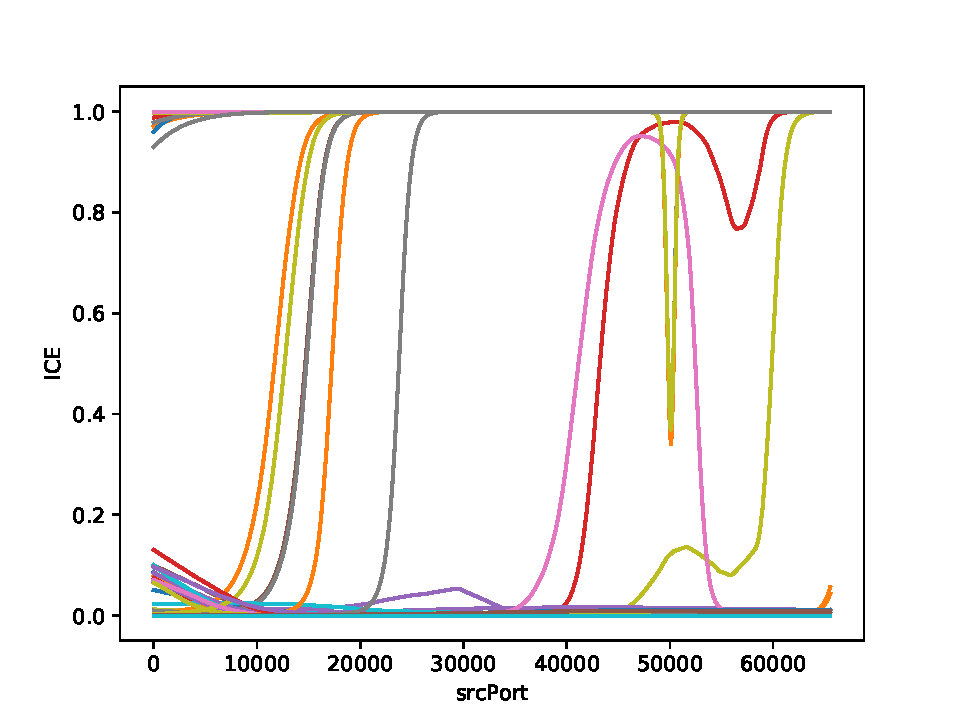
\includegraphics[width=0.48\textwidth]{../plots/pdp/sourceTransportPort_nn.pdf}
%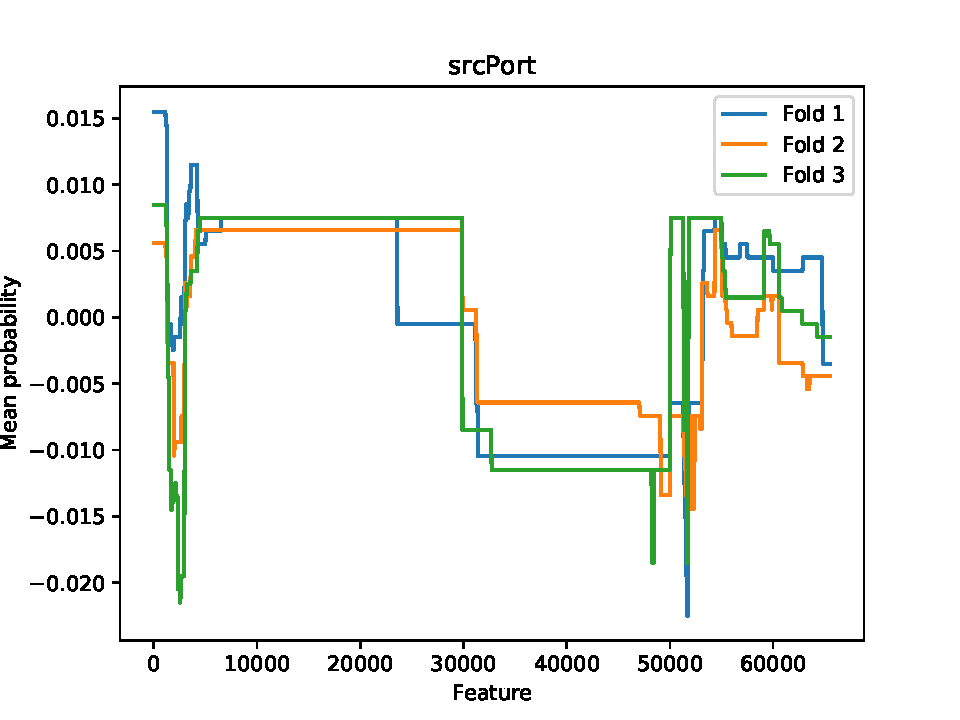
\includegraphics[width=0.48\textwidth]{../plots/pdp/sourceTransportPort_rf.pdf}
%
%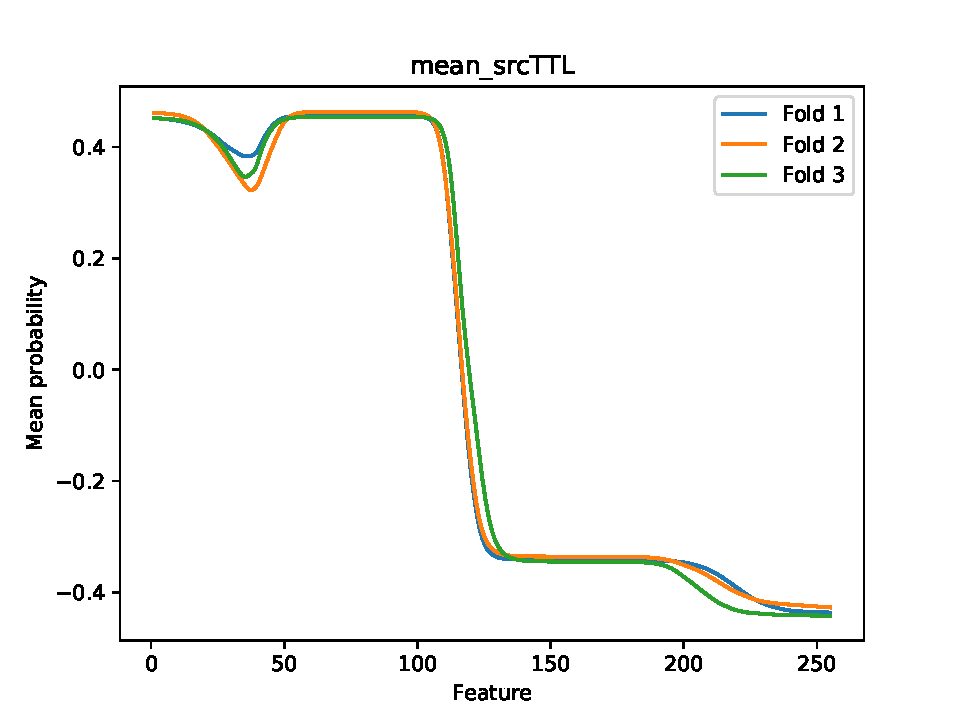
\includegraphics[width=0.48\textwidth]{../plots/pdp/apply(mean(ipTTL),forward)_nn.pdf}
%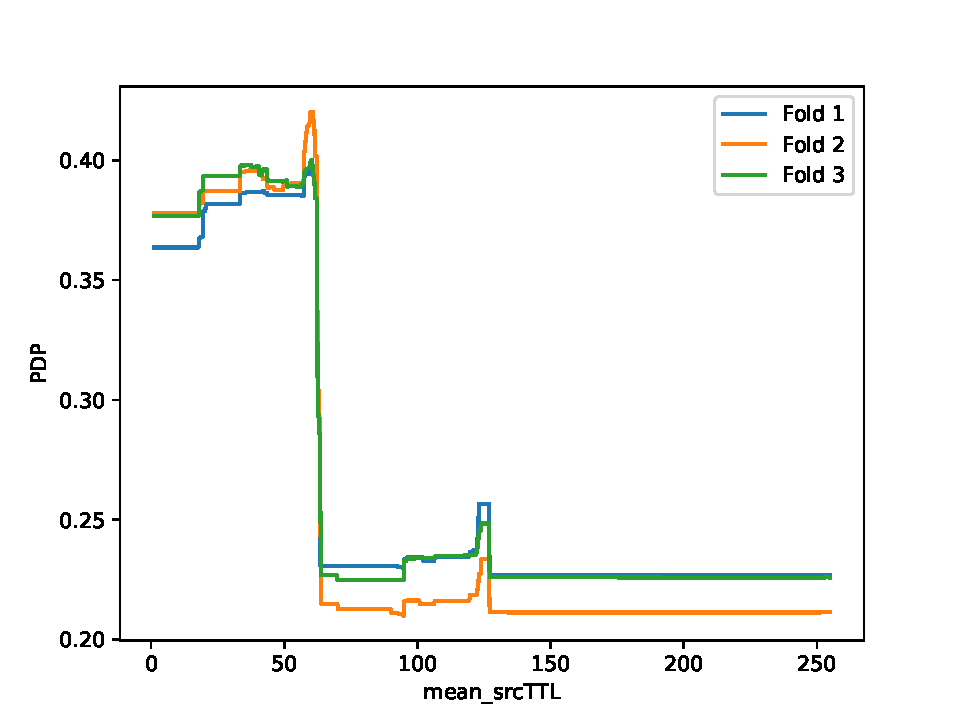
\includegraphics[width=0.48\textwidth]{../plots/pdp/apply(mean(ipTTL),forward)_rf.pdf}
%
%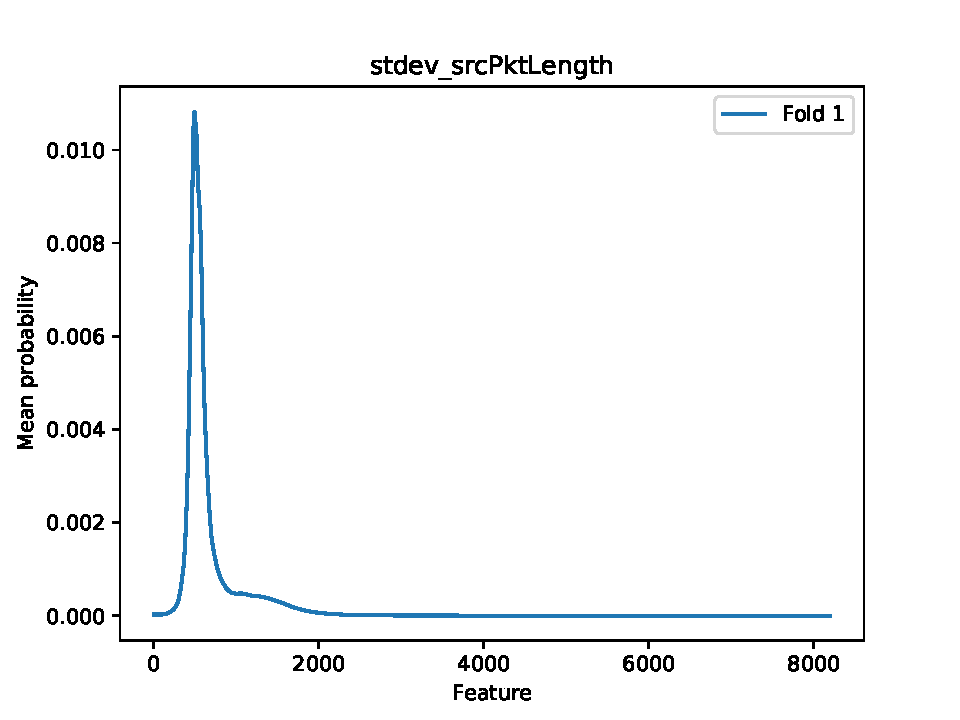
\includegraphics[width=0.48\textwidth]{../plots/pdp/apply(stdev(ipTotalLength),forward)_nn.pdf}
%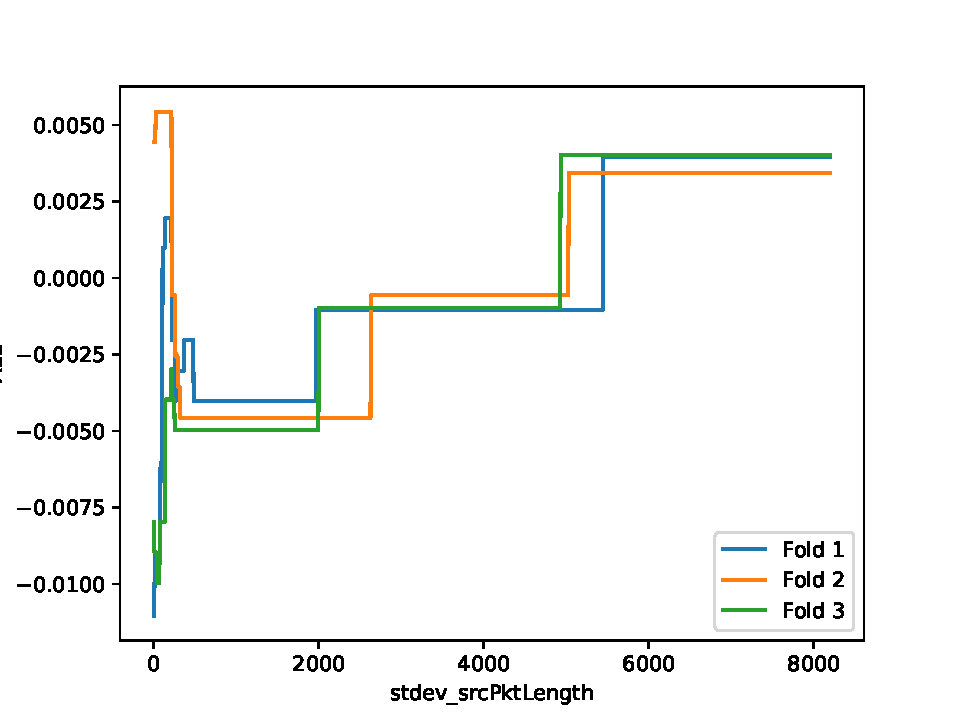
\includegraphics[width=0.48\textwidth]{../plots/pdp/apply(stdev(ipTotalLength),forward)_rf.pdf}
%
%\caption{Examples of conditional PD plots for source and destination port. We only analyze these features with the PDP since it is not straightforward to define the PDP for features that can vary for each packet in a flow.}
%\label{fig:pdp}
%\end{figure*}

In this variant of the PDP that we call conditional PDP, we don't take the whole dataset for the computation for the PDP but only a subset that belongs to a certain class. Specifically, we take each attack class and compute the PDP only over samples of this attack class. A known issue about PDPs in general is that dependencies of the feature under investigation and the remaining variables are not considered, hence potentially querying the neural network for feature combinations which cannot possibly occur. 

For this reason, Accumulated Local Effects (ALE) plots have been proposed in literature. The basic idea for ALE is that instead of using all samples, only the closest samples are used for assessing the effects of one feature. ALE plots therefore inherently require a distance measure for finding the closest samples, which, as revealed in the above discussion, in our case is not possible in a straight-forward manner.

\subsection{Plots for Sequences}

As apparent from the above discussion, trying to explain how packet features influence the model's predictions, poses various difficulties. As a first step to explaining our model's predictions, we investigate how important features at different time steps are for the model's decisions. Intuitively, features at the beginning of a flow should be the most important while the model's predictions should not vary significantly anymore, as soon as the model has come to a decision. 

%\begin{figure*}[p]
%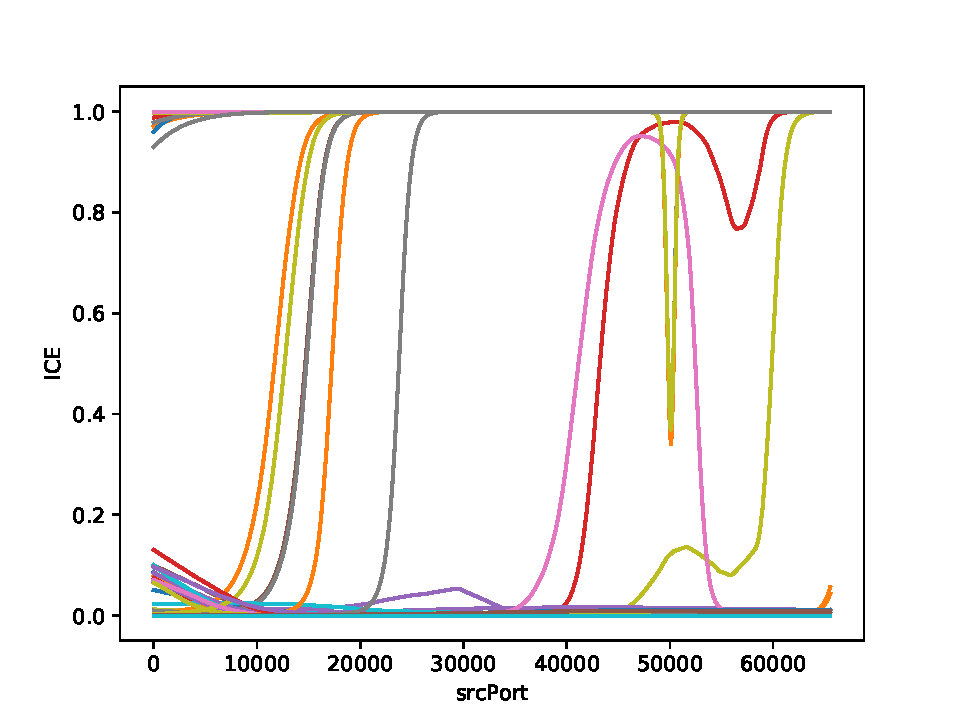
\includegraphics[width=0.48\textwidth]{../plots/pdp/sourceTransportPort_nn.pdf}
%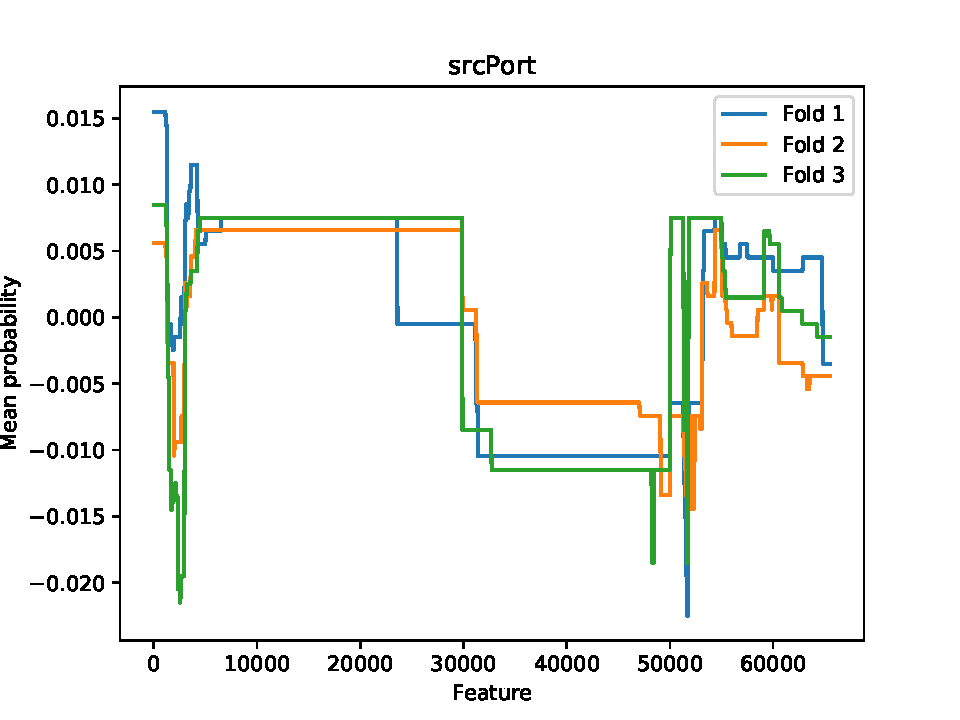
\includegraphics[width=0.48\textwidth]{../plots/pdp/sourceTransportPort_rf.pdf}
%
%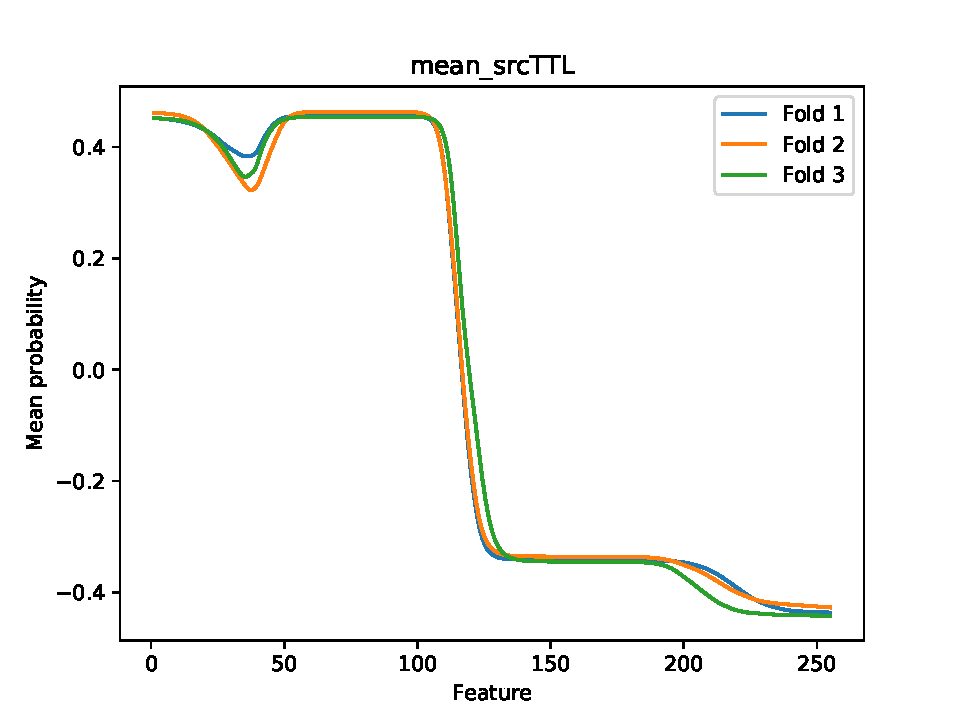
\includegraphics[width=0.48\textwidth]{../plots/pdp/apply(mean(ipTTL),forward)_nn.pdf}
%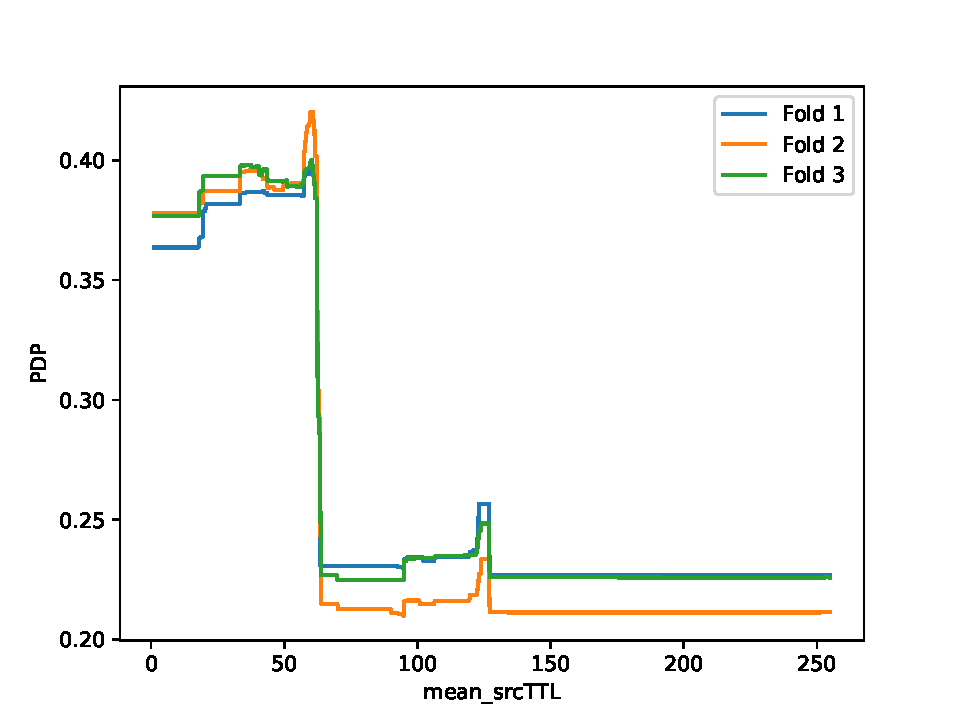
\includegraphics[width=0.48\textwidth]{../plots/pdp/apply(mean(ipTTL),forward)_rf.pdf}
%
%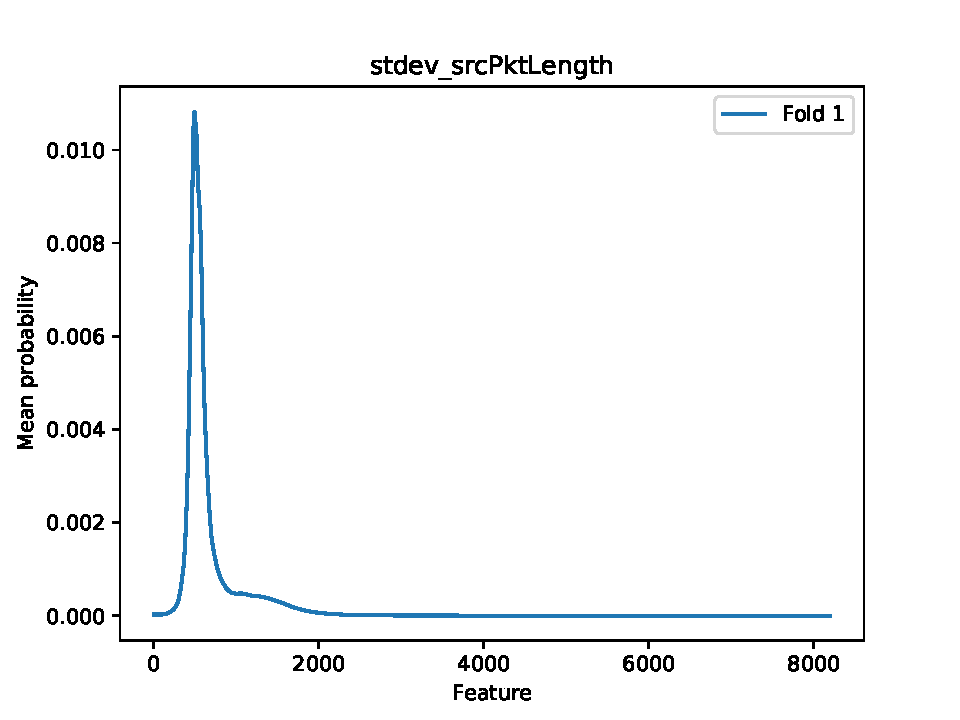
\includegraphics[width=0.48\textwidth]{../plots/pdp/apply(stdev(ipTotalLength),forward)_nn.pdf}
%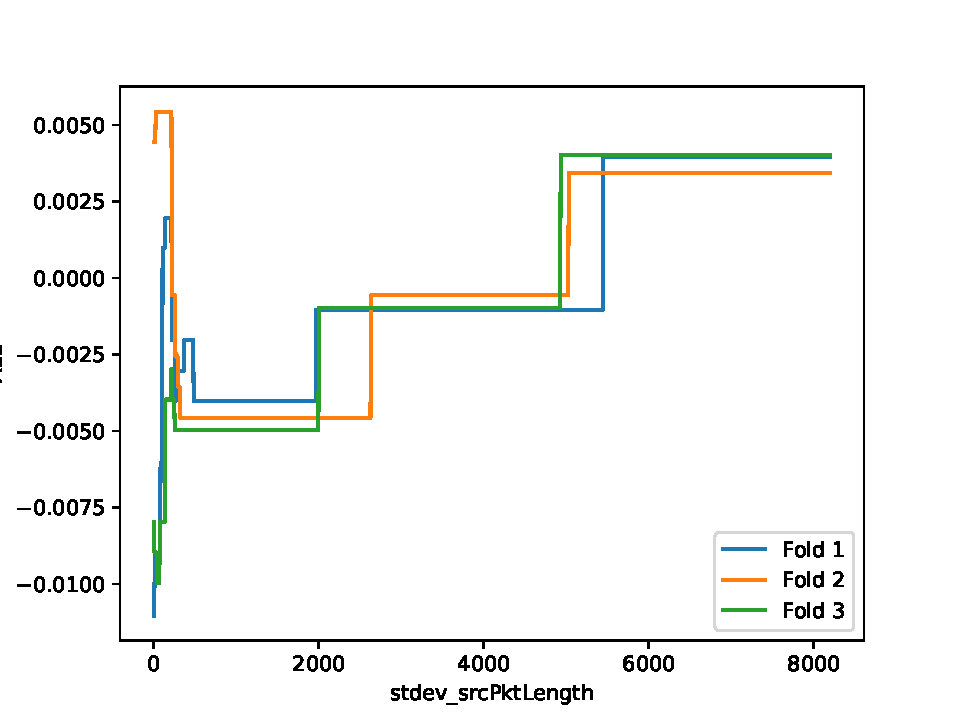
\includegraphics[width=0.48\textwidth]{../plots/pdp/apply(stdev(ipTotalLength),forward)_rf.pdf}
%
%\caption{Median confidence per time step and first and third quartiles for selected attack types. For the majority of attacks, confidence increases in the first few steps and then stays almost constant at 1.}
%\label{fig:pdp}
%\end{figure*}

To determine if this hypothesis is correct, we plot the attack confidence of the classifier for each time step for each attack class. At each time step we average over all flows and also show the first and third quartiles. \todo{Insert plots output and interpretation. Change plots to include a histogram.}

Next, we want to investigate if our classifier just memorized its inputs. The most interesting packet features to visualize to in our use case are the inter-arrival time (IAT) between packets in a flows and the packet length. To depict how the model comes to a decision, we determined the total minimum and maximum for these features. For a given flow $X$ we then varied feature values at each time step between minimum and maximum and determined the median, the first and the third quartile. \autoref{fig:predplots} shows several of such plots for different attack categories for IAT and packet length. Furthermore, the shades \autoref{fig:predplots2} depict the averaged predictions for different attack families. It seems clear that the classifier didn't just memorize the inputs but actually learned them since there is always a smooth decrease of confidence if we change the feature values. Instead, when memorizing, we would expect a sharp decline of confidence to occur. \todo{Insert pred\_plots2 output and interpretation}  

Looking at the plots of the features that vary over time we see that certain attack types have a characteristic pattern in which they send packets by which they are easily recognizable. We want to determine how the pattern of packet sizes and interarrival times is significant for the classification. Thus, we show the flow that is the easiest to classify for each attack type and the one that is the hardest to classify and check whether they are visually significantly different. \todo{Add characteristic\_flows output and add flow direction to the plots and explain the method.}

\section{Adversarial attacks}

As we saw in the previous section \todo{Add reference to characteristic\_flows plot here}, attacks do have a characteristic pattern of interarrival times and packet lengths. Thus,  changing this pattern might confuse the classifier. However, this scenario is quite different from how generating adversarial samples usually works: We have significantly less features than in, for example, an image. Furthermore, only two out of those few features can be manipulated. And even these features cannot manipulated freely: Besides the constraints that packet size and interarrival time cannot go beyond zero there are also more problem-specific constraints:
\begin{itemize}
\item Only packets can be manipulated which are transmitted by the attacker. This means the attacker can only control one direction (except for botnets where both sides are attackers). 
\item Packets must not be smaller than initially, as otherwise less information could be transmitted or packets might be rendered syntactically invalid.
\item Interarrival times must not decrease, as otherwise the physical speed of data transmission can be violated in some cases. Since an in-depth analysis of when the reduction of interarrival times is possible, would come with substantial effort, we generally disallowed a reduction of this feature.
\end{itemize}

Several methods for generating adversarial samples have been proposed in the recent literature, achieving different speed-quality tradeoffs. Since the reasons discussed above suggest that finding adversarial flows is particularly difficult in our case, for the present research we preferred methods which produces high-quality adversarial samples while not being as fast as other methods.

We implemented the following methods for generating adversarial flows.

\subsection{Carlini-Wagner}
In particular, we implemented the method by \citeauthor{carlini2017towards}~\cite{carlini2017towards}, which performs gradient descent on the optimization objective 
\begin{equation}
d(X,\tilde X) + \epsilon  \max(Z(\tilde X), 0).
\end{equation}
Here, $d(\cdot)$ is a distance metric, $\epsilon \in \mathbb R^+$ is a parameter governing the tradeoff achieved between attack success and distance from the original flow. Furthermore, $Z(\cdot)$ denotes the neural network's logit output, $X$ denotes the original flow and $\tilde X$ the adversarial flow under optimization. 

We used $\ell_1$ norm as distance metric and deployed projected gradient descent (PGD) for meeting the real-world constraints discussed above.

\subsection{$\ell_\infty$-bounded Projected Gradient Descent}
\cite{madry2017towards} use a method for generating adversarial samples which uses PGD  to minimize the network's negative loss function while constraining the achieved $\ell_\infty$ distance from the original samples. 

\subsection{Fast Gradient Sign Method}
Finally, we also tested the Fast Gradient Sign Method (FGSM), which was initially proposed in \cite{goodfellow2014explaining} and perhaps is the most frequently used method for generating adversarial sampling. FGSM can be considered a single pass of PGD on the loss function with an equality constraint on the $\ell_\infty$ distance, i.e. the adversarial sample is found as
\begin{equation}
\tilde X = X + \epsilon \text{sgn}( \nabla_X L(X)),
\end{equation}
where $L(X)$ denotes the network's loss function and $\epsilon$ denotes the achieved $\ell_\infty$ distance.

\subsection{Defences}

The most obvious defence, which is only possible because of the nature of the dataset, is to simply leave out features which the attacker can manipulate. For this, we try two different approaches: 
\begin{itemize}
\item Leaving out all features that are manipulable: packet size and interarrival time
\item Leaving out manipulable features when the attacker can manipulate them: only in the direction from the attacker to the victim (This, however does not prevent adversarial samples for botnets, for which both sides are malicious)
\end{itemize}

Both approaches lead to complete resistance to adversarial samples (as we left out all manipulable features), except for botnets, which can still operate when only leaving out manipulable features in one direction. The results in \autoref{performance_results_no_manipulable} show that -- surprisingly -- there is only a small difference in classification performance when only computing the accuracy for the last packet of each flow (flow accuracy). However, when looking at the packet accuracy, which considers all packets of all flows, there is a significant difference. Thus, apparently the interarrival time and packet size are especially important for determining whether a flow is malicious in the first packets of a flow. 

\begin{table*}
\caption{Comparing performance with all features, only safe features (interarrival time and packet size removed) and safe features in one direction (interarrival time and packet size removed for packets coming from source). \textit{packets} means that we consider the neural network output of all packets of the flow while \textit{flows} means that we only consider the last packet. At the last packet the classifier is usually already a lot more confident than at the first packets of a flow and thus metrics are always better in this case.}  \label{tab:performance_results_no_manipulable}
\newcommand{\cmidrulespace}{6pt}
\begin{tabular}{l l l l l l l} \toprule
& \multicolumn{2}{l}{all} & \multicolumn{2}{l}{safe features} & \multicolumn{2}{l}{safe features one direction} \\
\cmidrule(r){2-3} \cmidrule(lr){4-5} \cmidrule(l){6-7}
& packets & flows & packets & flows & packets & flows \\
\midrule
Accuracy & 0.9857054 & 0.99472587 & 0.96678023 & 0.99337596 & 0.98056073 & 0.99353386 \\
Precision & 0.94963342 & 0.9894422 & 0.87175275 & 0.98798596 & 0.91359787 & 0.98994595 \\
Recall & 0.96735895 & 0.98972051 & 0.94374958 & 0.98581328 & 0.97836672 & 0.9844478 \\
F1 & 0.95841423 & 0.98958134 & 0.90632359 & 0.98689842 & 0.94487366 & 0.98718922 \\
Youden & 0.95682951 & 0.98614231 & 0.91525628 & 0.98175163 & 0.95937772 & 0.9810602 \\
\bottomrule
\end{tabular}
\end{table*}

\section{Conclusions}

We have implemented a recurrent classifier based on LSTM to detect network attacks. While attack detection performance is not better than that of non-recurrent approaches, we can already detect attacks before they are over. Furthermore, the recurrent approach allows us to inspect the influence of single packets on the detection performance and shows which packets are \textit{characteristic} for attacks. 

We show that adversarial samples are possible even though the data we use are very different from those that are usually used when finding adversarial samples. 

\bibliographystyle{ACM-Reference-Format}
\bibliography{bibliography}


\end{document}
\endinput
%%
%% End of file `sample-sigconf.tex'.
